\documentclass{beamer}
\usepackage[utf8]{inputenc}
\usetheme{default}
\usecolortheme{dove}
\usepackage{textpos}
\usepackage{grid-system}
\usepackage[official]{eurosym}


% po4a: environment frame
% po4a: environment Row
% po4a: environment Cell


\title{Freifunk Darmstadt}
\author{
\includegraphics[width=4cm]{images/logo}}
%\institute[Inst.]{Freifunk Darmstadt}
\date{24. März 2015 | https://darmstadt.freifunk.net}

\begin{document}

\begin{frame}
\maketitle
\end{frame}

\addtobeamertemplate{frametitle}{}{%
\begin{textblock*}{100mm}(0.93\textwidth,-0.5cm)

\includegraphics[height=1cm]{images/logo}
\end{textblock*}}

%\begin{frame}{Themen}
%\tableofcontents
%\end{frame}

\section{Was ist Freifunk?}
\begin{frame}{Was ist Freifunk?}
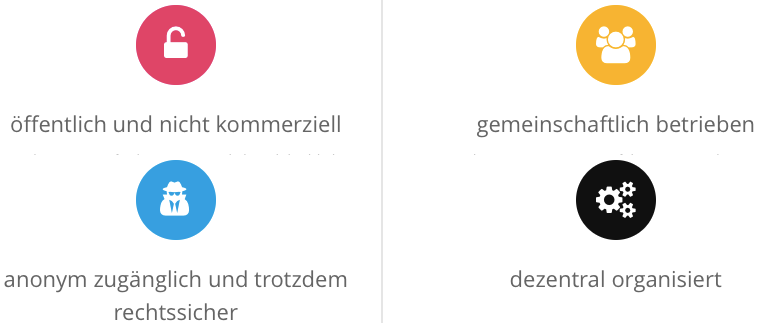
\includegraphics[width=1.1\textheight]{images/principles}$\;$
\begin{itemize}
	\item Teil einer weltweiten Bewegung für offene und freie Netze
	\item Internetzugang und Plattform für lokale Dienste
	\item dezentral und gemeinschaftlich betrieben
	\item robuste Netzwerktopologie durch Mesh-Netzwerk
	\item Freifunk Darmstadt: Initiative der HG Chaos Darmstadt e.V.
\end{itemize}
\end{frame}


\begin{frame}{Freifunk in Darmstadt}
\vfill
\begin{center}
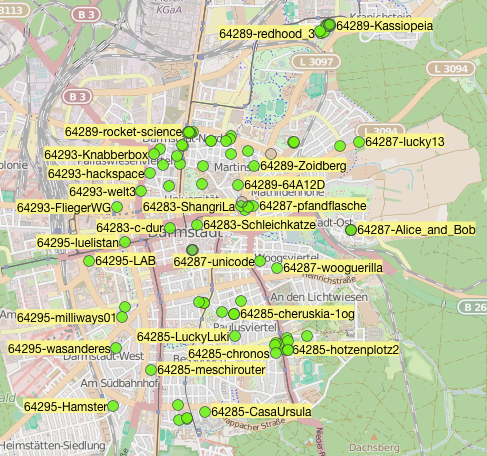
\includegraphics[height=0.8\textheight]{images/map3-15}$\;$
%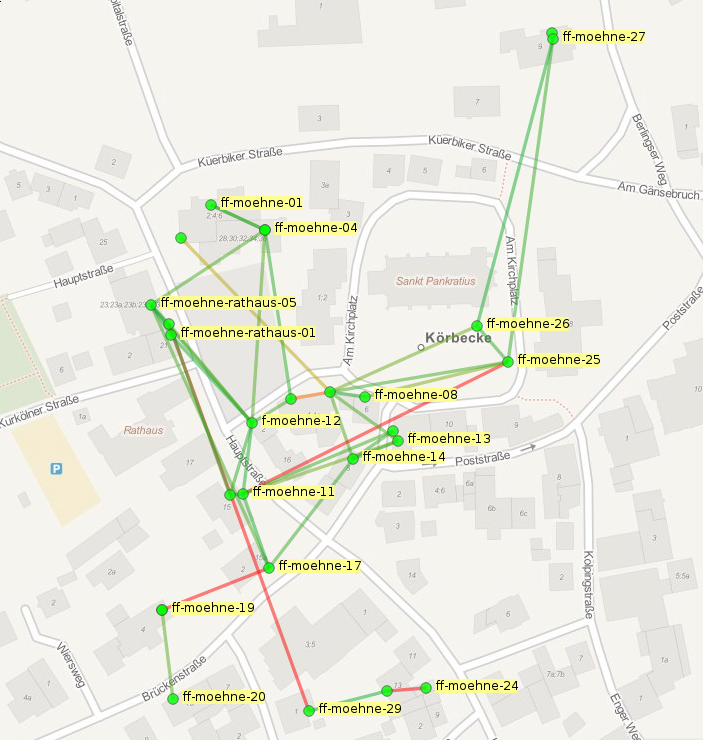
\includegraphics[height=0.6\textheight]{images/moehne}
https://map.darmstadt.freifunk.net
\end{center}
\vfill
\end{frame}

\section{Projektbeschreibung}
\begin{frame}{Projektbeschreibung}
\vfill
\begin{center}
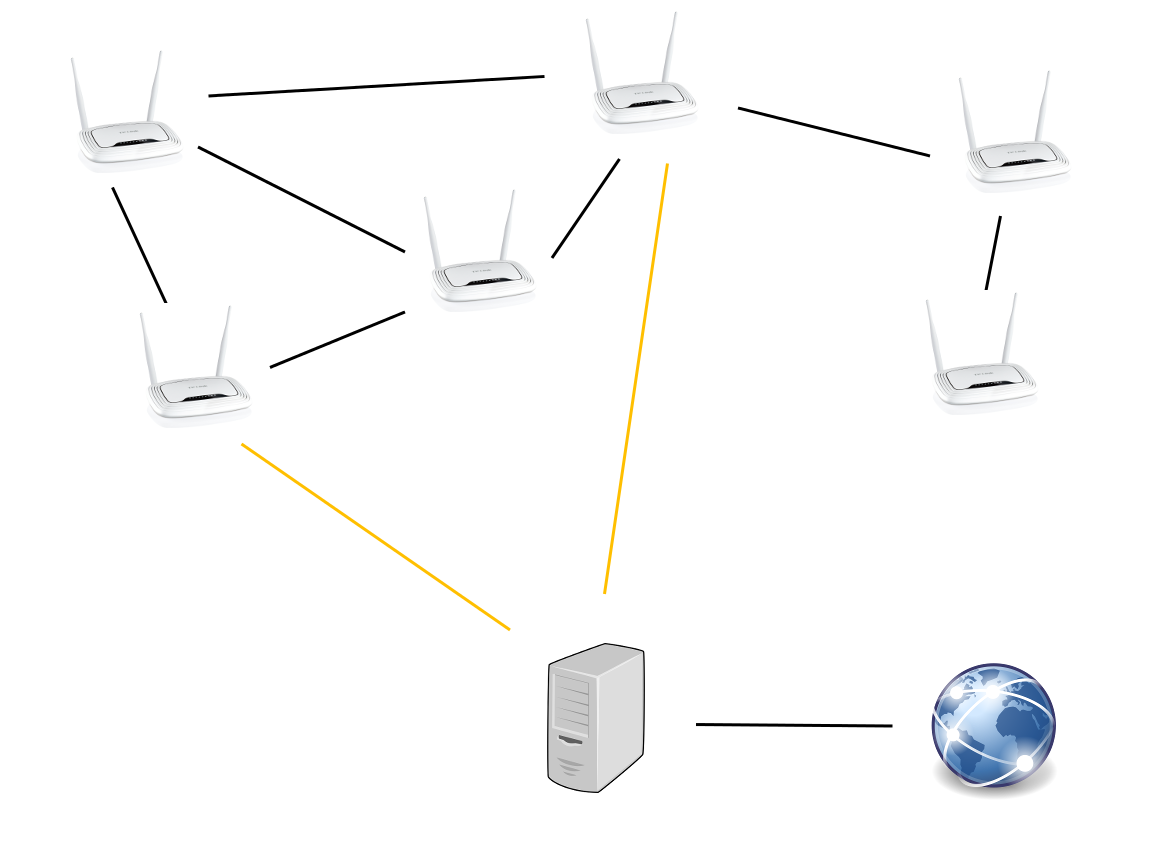
\includegraphics[height=0.7\textheight]{images/meshing}
\end{center}
\vfill
\end{frame}


\begin{frame}{Mitmachen!}
\vfill
\begin{center}
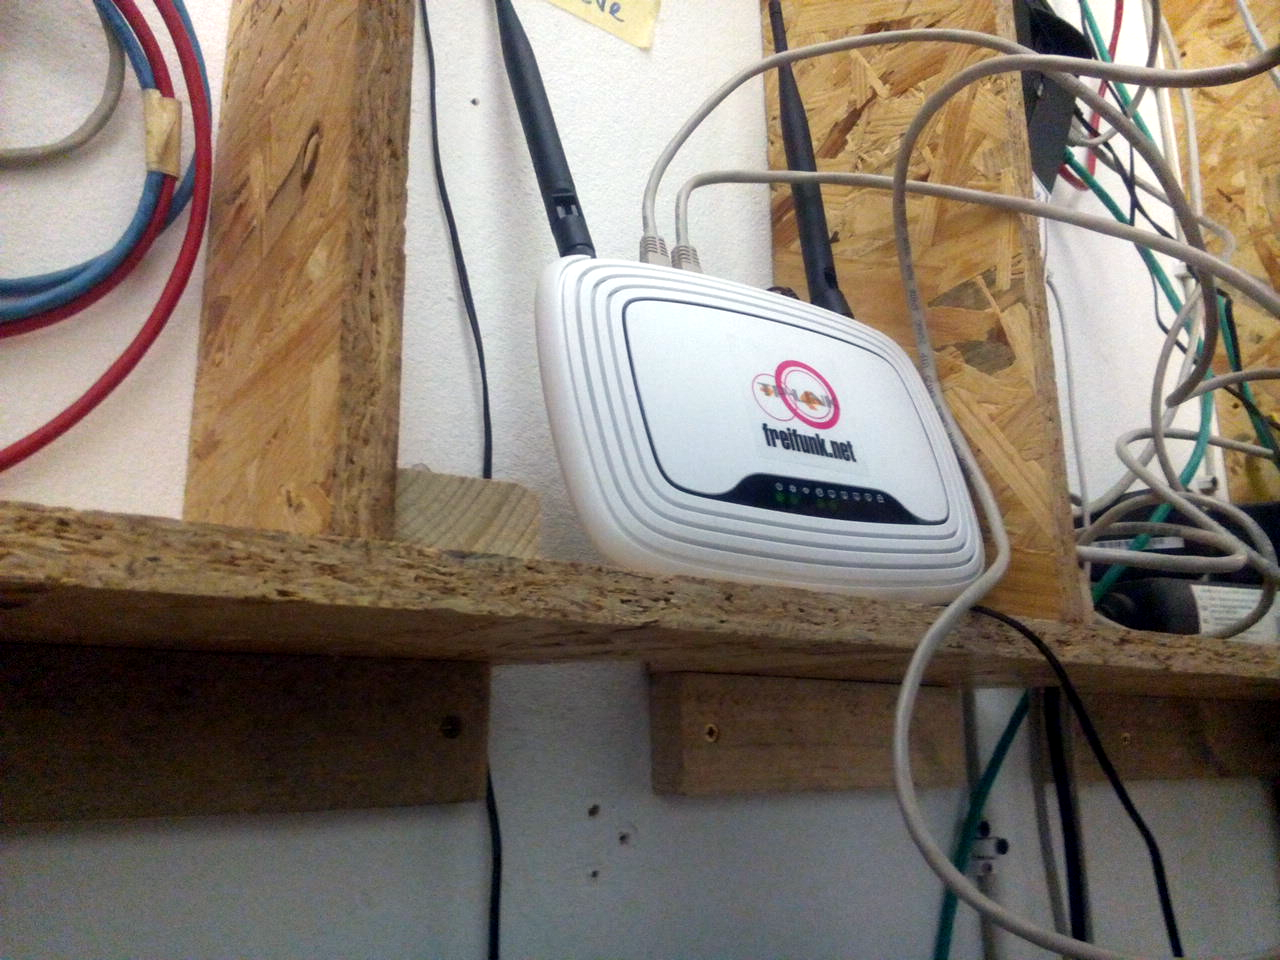
\includegraphics[height=0.5\textheight]{images/irl_router}$\;$
\vfill
Flyer am Ausgang \\
https://darmstadt.freifunk.net
\end{center}
\end{frame}

\end{document}
